\section{Theorie}

\subsection{Einleitung und Erklärung der Dampfdruckkurve und der Verdampfungswärme }

\begin{flushleft}
    Unter einer Phase wird ein räumlich abgegrenzter Bereich in einem abgeschlossenem System, in welchem ein Stoff einen physikalisch homogenen Zustand hat, verstanden.
    Aggregatzustände sind demnach auch Phasen, welche als flüssig, gasförmig oder fest vorhanden sein können.
    Bei diesem Versuch wird die Umwandlung von flüssig zu gasförmig und umgekehrt betrachtet und näher untersucht.
    In einem Zustandsdiagramm, wie in Abbildung \ref{Abbildung1} zu sehen, kann das Verhältnis der Phase gut beschrieben werden.
    Dabei werden zwei sogenannte Freiheitsgrade betrachtet, welche in diesem Fall Temperatur $T$ und Druck $p$ sind.
\end{flushleft}

\begin{figure}[H]  
    \centering
    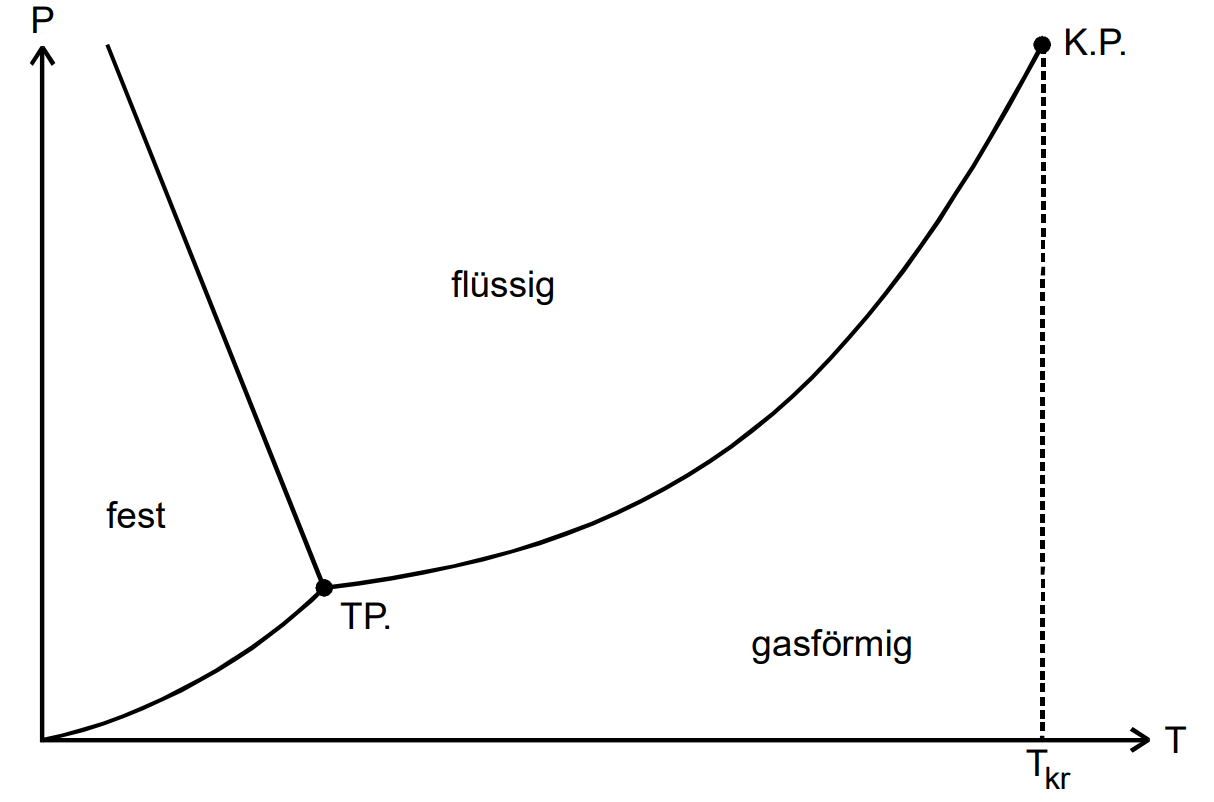
\includegraphics[width=110mm]{bilder/Zustandsdiagramm.png}
    \caption{Das Zustandsdiagramm mit den 3 Phasen \cite{a1}. \label{Abbildung1} }
\end{figure}

\begin{flushleft}
    Da in diesem Versuch die Umwandlung von flüssig zu gasförmig und umgekehrt relevant ist, fällt der Fokus auf die Kurve von TP.,den Tripelpunkt, zu K.P., dem kritischen Punkt.
    Der Tripelpunkt ist der Punkt an dem die drei Phasen gleichzeitig vorliegen und der kritische Punkt ist der Punkt an dem die flüssige, sowie die gasförmige Phase des Wassers gleichzeitig vorhanden ist.
    Diese Kurve, die beide Punkte verbindet, wird auch Dampfdruckkurve genannt.
    In diesem Fall sind die beiden Freiheitsgrade nicht mehr frei wählbar. Bei einer bestimmten Temperatur $T$ ist der Druck $p$ durch die Dampfdruckkurve gegeben.
    Somit minimiert sich der Freiheitsgrad auf eins, und zwar $T$. 
    Der Verlauf der Dampfdruckkurve ist durch einen temperaturabhängigen Parameter, welcher in einigen Bereichen jedoch als konstant betrachtet wird, festgelegt. 
    Diese Größe wird als Verdampfungswärme $L$ gekennzeichnet.
    Diese Größe verschwindet, je näher der Verlauf der Kurve sich dem kritischem Punkt nähert,weil an diesem Punkt kein Unterschied mehr zwischen diesen Phasen existiert.
    Der Wert bei dem $L$ als praktisch konstant angenommen wird, wird mithilfe dieses Experimentes ermittelt und die dazugehörige Dampfdruckkurve bestimmt.
\end{flushleft}

\subsection{}

\begin{flushleft}
    Wenn in ein evakuiertes Gefäß, Flüssigkeit hinzugefügt wird steigt der Druck überhalb der Wasseroberfläche, aufgrund des Verdampfens von einem Teil der Flüssigkeitsmenge, an.
    Unter dem Verdampfungsvorgang wird das Verlassen der auf der Flüssigkeitsoberfläche befindenden Moleküle, welche nach der Maxwellschen Geschwindigkeitsverteilung eine maximale kinetische Energie besitzen, verstanden.
    Dabei wird Arbeit gegen die Molekularkräfte aufgewandt, welche entweder durch von außen zugeführte Energie oder die Entnahme des Wärmevorrats der Flüssigkeit, erbracht wird. 
    Die molare Verdampfungswärme $L$ ist hierbei die Energie, mit der ein Mol an Flüssigkeit in gleichwarmen Dampf umgewandelt wird. 
    Ebenfalls kommt die Energie bei Kondensation, also dem umgekehrten Vorgang, wieder frei, aufgrund der Maxwellschen Geschwindigkeitsverteilung.
    Der Druck der entsteht, wenn nach einiger Zeit ein Gleichgewicht zwischen Verdampfung und Kondensation herrscht, wird Sättigungsdruck genannt.
    Dadurch, dass der Sättigungsdruck unabhängig vom Volumen des Gasraumes ist, kann dieser nicht durch die ideale Gasgleichung
\end{flushleft}

\begin{equation}
    pV = RT \label{1}
\end{equation}

\begin{flushleft}
    bestimmt werden. Das $R$ steht hierbei für die allgemeine Gaskonstante welche $8,314\, \frac{\text{J}}{\text{mol\,K}}$ beträgt.
\end{flushleft}

\subsection{Herleitung der Berechnung von der Dampfdruckkurve}

\begin{flushleft}
    Zu Beginn wird erst einmal der reversiblen Kreisprozess der Verdampfung und Kondensation betrachtet.
\end{flushleft}

\begin{figure}[H]       
    \centering
    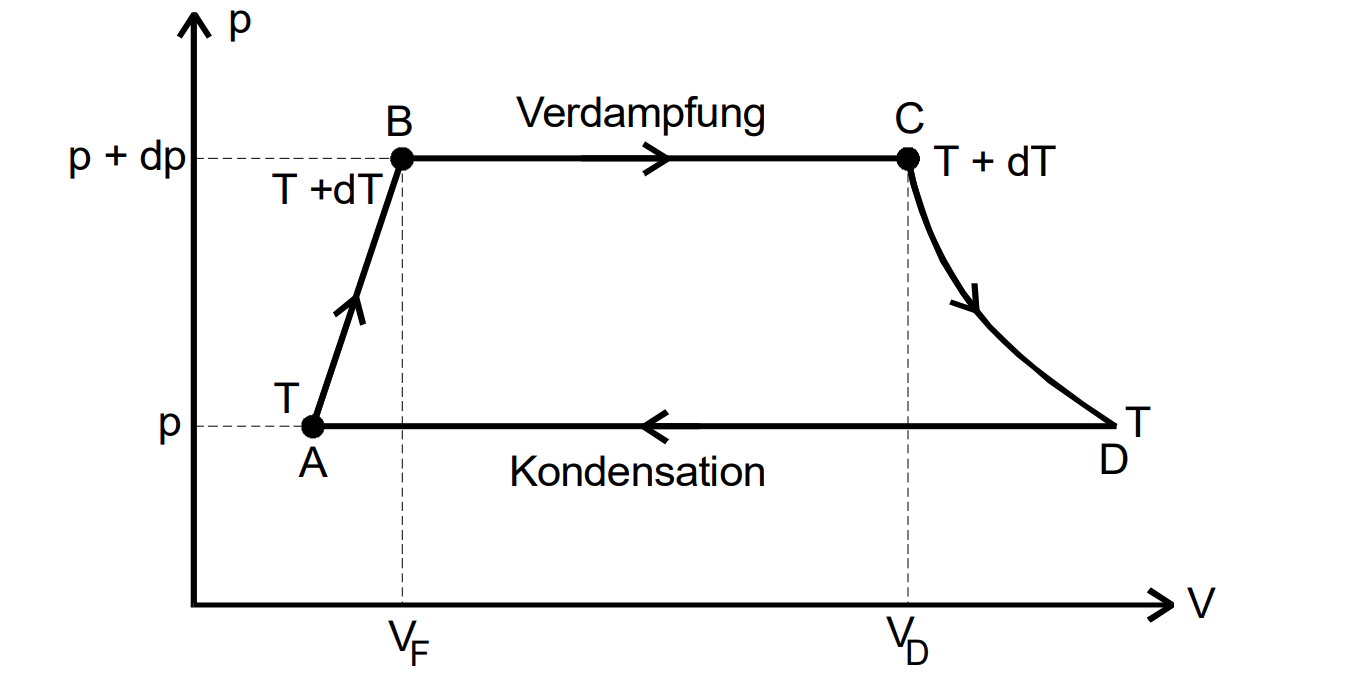
\includegraphics[height=65mm]{bilder/Kreisprozess.png}
    \caption{Der Kreisprozess in einem Druck-Volumen-Diagramm \cite{a1}. \label{Abbildung2} }
\end{figure}

\begin{flushleft}
    Der Verlauf startet bei dem Ausgangszustand \textbf{A}, sowie der Temperatur $T$ und dem Druck $p$.
    Die Flüssigkeit wird dann um eine Temperatur d$T$ erhitzt, wodurch dann ebenfalls der Druck um d$p$ auf ein Volumen $V_{\text{F}}$ steigt, Zustand \textbf{B}.
    Durch Zufuhr von Verdampfungswärme wird die Flüssigkeit isotherm und isobar und geht in eine Gasform über.
    Das Volumen dehnt sich dabei auf $V_{\text{D}}$ aus , Zustand \textbf{C}.\\
    \vspace{0.3cm}
    Der Dampf kühlt sich dann anschließend wieder auf die Ausgangstemperatur $T$ ab, mit dem Ausgangsdruck $p$, Zustand \textbf{D}.
    Die darauffolgende Kondensation erfolgt dann durch Zufuhr mechanischer Energie und gelangt somit wieder zum Ausgangszustand \textbf{A}.
    Die ganzen Prozesse werden nun aufeinander summiert und mit der gesamtverrichteten Arbeit gleichgesetzt, erster Hauptsatz der Thermodynamik, wodurch man folgende Gleichung erhält:
\end{flushleft}

\begin{equation}
    (C_{\text{F}} - C_{\text{D}}) \text{d}T + \text{d}L = (V_{\text{D}} - V_{\text{F}})\text{d}p\,. \label{2}
\end{equation}

\begin{flushleft}
    Die Parameter $C_{\text{F}}$ und $C_{\text{D}}$ geben die Molwärme des Dampfes an und d$L$ gibt den Unterschied der benötigten Verdampfungswärme an, da bei höheren Temperaturen die Unterschiede kleiner sind.
    Dadurch, dass dies ein reversibler Kreisprozess ist, gilt nach dem zweiten Hauptsatz der Thermodynamik
\end{flushleft}

\begin{align}
    \sum \limits_{i} \frac{Q_{i}}{T_{i}} = 0\,. \label{3}
    \intertext{Durch Umformen und die Formeln (\ref{2}) und (\ref{3}) ergibt sich die Clausius-Clapeyronsche Gleichung}
    (V_{\text{D}} - V_{\text{F}})\,\,\text{d}p = \frac{L}{T}\,\,\text{d}T\,.  \label{4}
\end{align}

\subsection{Die Anwendung der Clausius-Clapeyronsche Gleichung }

\begin{flushleft}
    Durch die Clausius-Clapeyronsche Gleichung kann nun die Berechnung der Dampfdruckkurve erfolgen, jedoch muss diese erst weiter vereinfacht werden, da Werte wie $V_{\text{D}}$, $V_{\text{F}}$ und L prinzipiell aus schwierigen Funktionen der Temperatur sein können. \\
    \vspace{0.3cm}
    Deswegen wird diese etwas vereinfacht, indem über die Temperaturbereiche, der vorher genannten Werte, Näherungsannahmen getroffen.
    Die getroffen Annahmen sind, dass $V_{\text{F}}$ gegenüber $V_{\text{D}}$ vernachlässigbar ist, $V_{\text{D}}$ sich mit der idealen Gasgleichung (\ref{1}) berechnen lässt und $L$ temperatur- und druckunabhängig ist.
\end{flushleft}

\begin{align}
    \intertext{Durch diese Annahmen und Integration folgt die Formel}
    \ln(p) = -\frac{L}{RT} + \text{const} \label{5}
    \intertext{bzw.}
    p = p_{0} \cdot e^{-\frac{L}{RT}}\,. \notag
\end{align}